The following User-Interface flow diagram enable us to model the high-level relationships between major user interface elements that are described in our RASD documents. It is used to organize the activities of TrackME application into groups and have an overview of the interfaces and interactions. \newline

\begin{itemize}
\item The user interface for an individual allows the individual to view the vitals, view the third party details, and accept/reject the request.
\begin{figure}[H]
	\begin{center}
		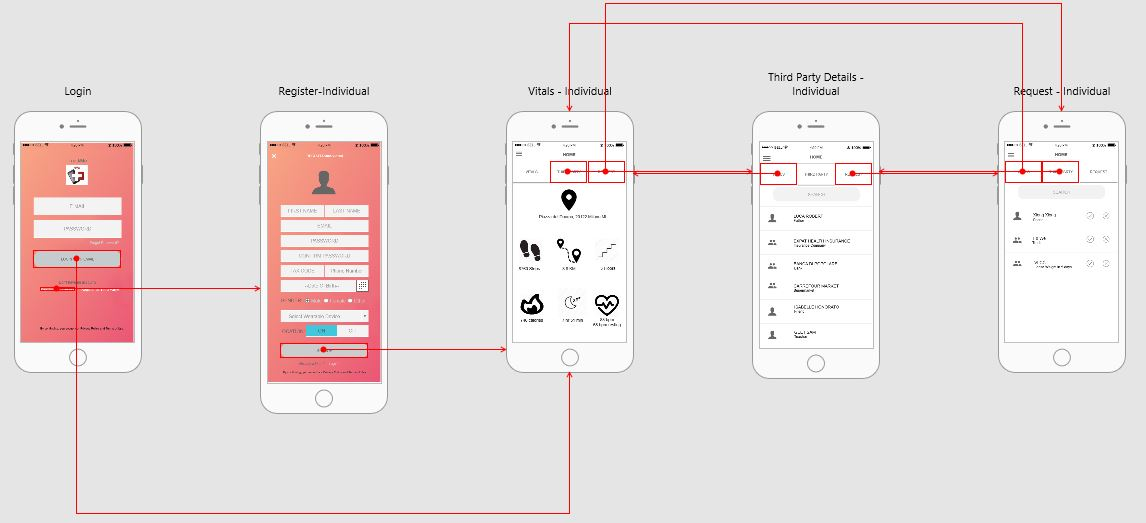
\includegraphics[width=\textwidth]{./DD_Diagrams/UI_Individual.JPG}
        \caption{User Interface - Individual}
        \label{ui_individual}
	\end{center}
\end{figure}
\end{itemize}

\begin{itemize}
\item The user interface for a Third Party allows the third party to view the details of the individual viewed in a pop-up box, allows to make new request, and view the status of the request already made.
\begin{figure}[H]
	\begin{center}
		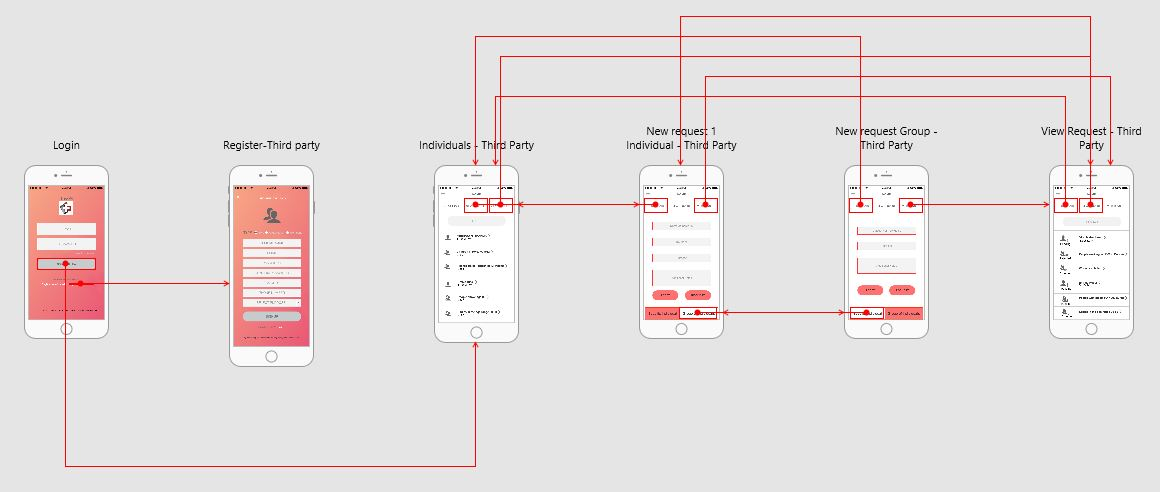
\includegraphics[width=\textwidth]{./DD_Diagrams/UI_ThirdParty.JPG}
        \label{ui_thirdparty}
        \caption{User Interface - Third Party}
	\end{center}
\end{figure}
\end{itemize}

\begin{itemize}
\item The Menu Interface allows an user to view their own profile, upgrade to a new service, and then allow to view the new service.
\begin{figure}[H]
	\begin{center}
		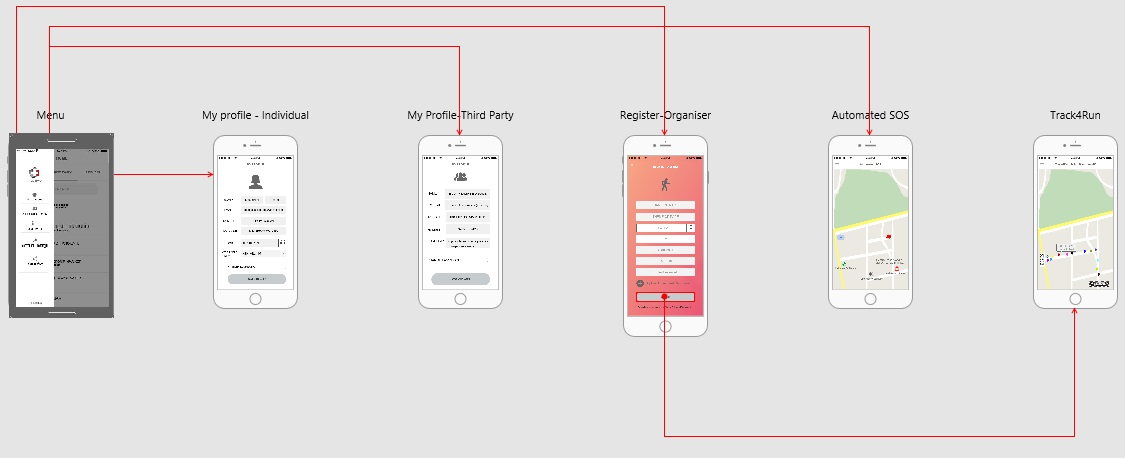
\includegraphics[width=\textwidth]{./DD_Diagrams/UI_Menu.JPG}
        \caption{User Interface - Menu}
        \label{ui_menu}
	\end{center}
\end{figure}
\end{itemize}
